\documentclass[journal]{IEEEtran}
\usepackage[T1]{fontenc}
\usepackage{amsmath,amssymb,array,booktabs,url,microtype,graphicx,float}
\graphicspath{{figures/}}
\usepackage[scaled=0.88]{newtxtt}
\newcommand{\pp}{\,\mathrm{pp}}
\renewcommand{\thesection}{S-\Roman{section}}
\renewcommand{\thetable}{S\arabic{table}}
\renewcommand{\thefigure}{S\arabic{figure}}
\usepackage[colorlinks=true,linkcolor=blue,urlcolor=blue]{hyperref}
\begin{document}
\title{Supplementary Material: Cross-Track Sentinel-1 Land-Cover Classification with Two-Acquisition Interferometric Coherence}
\author{Shiji Fan, Daniel Albuquerque, Pedro Pinho, and Ming Shen}
\maketitle
\section{Source-Track Model Selection}
Tables~\ref{tab:hp_rf} and~\ref{tab:hp_svc} list the 40 configurations selected by buffered source-track spatial cross-validation. Each configuration is then fitted with training-sample seeds 17, 29, and 43. The RF uses 300 trees; the SVC uses an RBF kernel and a source-fitted robust scaler. SVC entries report the multiplier of $\gamma_{\mathrm{scale}}$. The displayed validation accuracy is the mean across the three source spatial folds.
\begin{table}[!t]\centering\footnotesize
\caption{RF configurations selected with 400\,m spatial exclusion.}\label{tab:hp_rf}
\setlength{\tabcolsep}{3pt}\begin{tabular}{llrrr}\toprule
Repr. & Track & $m_{\rm features}$ & Min. leaf & CV BA (\%) \\\midrule
$I_8$ & T15 & $\sqrt{D}$ & 1 & 68.06 \\
$I_8$ & T37 & $\sqrt{D}$ & 1 & 68.84 \\
$I_8$ & T88 & 0.5 & 1 & 67.48 \\
$I_8$ & T139 & 0.5 & 1 & 69.35 \\
$I_{28}$ & T15 & 0.5 & 1 & 70.74 \\
$I_{28}$ & T37 & $\sqrt{D}$ & 1 & 71.85 \\
$I_{28}$ & T88 & 0.5 & 1 & 69.99 \\
$I_{28}$ & T139 & $\sqrt{D}$ & 1 & 72.95 \\
$I_8+g_{12}$ & T15 & $\sqrt{D}$ & 1 & 77.52 \\
$I_8+g_{12}$ & T37 & 0.5 & 1 & 76.58 \\
$I_8+g_{12}$ & T88 & 0.5 & 1 & 75.81 \\
$I_8+g_{12}$ & T139 & $\sqrt{D}$ & 1 & 77.32 \\
$F_{12}$ & T15 & 0.5 & 1 & 77.81 \\
$F_{12}$ & T37 & $\sqrt{D}$ & 1 & 77.07 \\
$F_{12}$ & T88 & $\sqrt{D}$ & 1 & 74.13 \\
$F_{12}$ & T139 & 0.5 & 5 & 77.47 \\
$I_{28}+g_{12}$ & T15 & 0.5 & 1 & 78.08 \\
$I_{28}+g_{12}$ & T37 & 0.5 & 1 & 77.86 \\
$I_{28}+g_{12}$ & T88 & $\sqrt{D}$ & 1 & 75.99 \\
$I_{28}+g_{12}$ & T139 & $\sqrt{D}$ & 1 & 78.39 \\
\bottomrule\end{tabular}\end{table}
\begin{table}[!t]\centering\footnotesize
\caption{SVC configurations selected with 400\,m spatial exclusion.}\label{tab:hp_svc}
\setlength{\tabcolsep}{3pt}\begin{tabular}{llrrr}\toprule
Repr. & Track & $C$ & $\gamma$ multiplier & CV BA (\%) \\\midrule
$I_8$ & T15 & 100.0 & 0.1 & 66.95 \\
$I_8$ & T37 & 10.0 & 0.1 & 68.12 \\
$I_8$ & T88 & 1.0 & 1.0 & 66.28 \\
$I_8$ & T139 & 100.0 & 0.1 & 68.83 \\
$I_{28}$ & T15 & 1.0 & 0.1 & 70.44 \\
$I_{28}$ & T37 & 10.0 & 0.1 & 71.04 \\
$I_{28}$ & T88 & 10.0 & 0.1 & 69.46 \\
$I_{28}$ & T139 & 100.0 & 0.1 & 72.12 \\
$I_8+g_{12}$ & T15 & 10.0 & 0.1 & 79.73 \\
$I_8+g_{12}$ & T37 & 10.0 & 0.1 & 77.38 \\
$I_8+g_{12}$ & T88 & 10.0 & 0.1 & 76.08 \\
$I_8+g_{12}$ & T139 & 10.0 & 0.1 & 77.13 \\
$F_{12}$ & T15 & 10.0 & 0.1 & 79.32 \\
$F_{12}$ & T37 & 10.0 & 0.1 & 77.44 \\
$F_{12}$ & T88 & 100.0 & 0.1 & 75.61 \\
$F_{12}$ & T139 & 10.0 & 0.1 & 77.07 \\
$I_{28}+g_{12}$ & T15 & 10.0 & 0.1 & 80.33 \\
$I_{28}+g_{12}$ & T37 & 10.0 & 0.1 & 77.90 \\
$I_{28}+g_{12}$ & T88 & 10.0 & 0.1 & 77.91 \\
$I_{28}+g_{12}$ & T139 & 100.0 & 0.1 & 78.19 \\
\bottomrule\end{tabular}\end{table}
\section{Label and Support Sensitivity}
The label sensitivity experiment uses the primary training and evaluation blocks with a separate sample on $U_2$, the support with valid labels in both products. Up to 800 pixels per evaluation block are drawn with seed $42+b$, where $b$ is the block identifier. Restricting this sample to product agreement defines its $C_2$ subset. Training candidates within 400\,m of any sampled evaluation pixel are excluded; each final fit uses 20,000 pixels and the frozen source-track hyperparameters. Thus, the $C_2$ sensitivity sample differs from the primary 9,600-pixel consensus sample.

WorldCover (WC), CORINE (CLC), and consensus labels are combined into six training--evaluation designs. Table~\ref{tab:label_full} reports mean paired increments over twelve directed track pairs and three sampling seeds. Bracketed values are the empirical 2.5th and 97.5th percentiles of these 36 deployment increments. They describe variation among the evaluated deployments and are not confidence intervals for a population mean. Primary spatial block-bootstrap intervals are reported separately in the main article.
\begin{table*}[!t]\centering\small
\caption{Buffered label/support sensitivity: mean $\Delta$BA and central 95\% deployment range (pp).}
\label{tab:label_full}
\begin{tabular}{lllrr}\toprule
Training label & Evaluation label & Support & RF & SVC \\\midrule
WC & WC & U2 & +3.64 [0.68, 6.79] & +6.68 [3.95, 10.02] \\
WC & CLC & U2 & +5.54 [2.97, 7.92] & +8.76 [5.04, 12.61] \\
CLC & CLC & U2 & +6.53 [4.61, 9.56] & +8.46 [5.59, 13.67] \\
CLC & WC & U2 & +4.14 [2.28, 6.73] & +5.69 [2.61, 10.09] \\
WC & WC & C2 & +6.96 [4.37, 10.66] & +11.07 [6.73, 15.96] \\
C2 & C2 & C2 & +7.02 [4.21, 10.45] & +7.60 [3.79, 11.07] \\
\bottomrule\end{tabular}\end{table*}

\section{Spatial Resampling and Temporal Evaluation}
Primary spring contrasts use a paired bootstrap of twelve evaluation blocks with replacement. Each draw uses the same block multiplicities for the compared representations, tracks, and seeds. Of 20,000 draws, 19,306 contain all five classes; spring BA intervals use this subset. The other 694 draws omit water. The evaluation sample contains 1,935 forest, 5,302 grassland, 2,140 cropland, 165 built-up, and 58 water pixels.

The autumn analysis uses the frozen spring RF and SVC models for $I_{28}$ and $I_{28}+g_{12}$, yielding 48 fitted model configurations and 1,843,200 prediction rows across all targets. No autumn labels enter model fitting or selection. Cross-track metrics exclude each model's source-track target. The prediction table contains 9,600 unique evaluation pixels.

The autumn bootstrap retains all 20,000 block draws. In the 633 draws with an absent class, BA averages recall over classes present in both compared arms. BA intervals are bias-corrected and accelerated (BCa), using leave-one-block-out estimates for acceleration; OA intervals are percentile intervals. Table~\ref{tab:autumn} reports full-sample point estimates separately from bootstrap summaries.
\begin{table}[!t]\centering\footnotesize
\caption{Autumn paired increments and 95\% intervals (pp).}\label{tab:autumn}
\begin{tabular}{llrr}\toprule
Model & Metric & Increment & Interval \\\midrule
RF & BA & 5.03 & [3.33, 7.08] \\
SVC & BA & 5.23 & [3.36, 7.27] \\
RF & OA & 0.62 & [-0.36, 1.74] \\
SVC & OA & -0.01 & [-0.68, 0.79] \\\bottomrule
\end{tabular}\end{table}

\section{Radiometric Processing Convention}
RTC products are converted to a common dB representation before interpolation to the analysis grid. T15 and T37 products are delivered in dB; T88 and T139 products are delivered in linear power. The latter undergo $10\log_{10}$ conversion at native resolution before bilinear interpolation to 40\,m. This order applies the same radiometric operation across tracks. Conversion after interpolation would yield a different result because logarithms and spatial averaging do not commute. The processing implementation is retained in \texttt{sar\_v2/data/}\allowbreak\texttt{build\_4track\_cube\_LOCAL\_v3.py}.

\section{Geographic Replication Feasibility}
The campaign records two Friesland candidate boxes: Box A spans $5.30$--$5.85^\circ$E and $52.80$--$53.20^\circ$N; Box B spans $5.30$--$5.84^\circ$E and $53.00$--$53.40^\circ$N. The archive-query record reports that T139 does not cover these candidates. Reproducing the Site-1 configuration would therefore require a different orbit set. The geographic evaluation remains unexecuted; the reported external acquisition experiment is the same-site autumn evaluation. The candidate definitions and coverage issue are recorded in \texttt{external\_validation/}\allowbreak\texttt{NEEDS\_AUTHOR\_DECISION.md}.

\section{Artifact Map}
Paths below are relative to the project root. The primary campaign directory is \texttt{tgrs\_final\_campaign\_20260915}.
\begin{itemize}\raggedright
\item Main models and pixel predictions: campaign \texttt{runs\_R1/}.
\item Selected parameters: campaign \texttt{configs/R1\_selected\_models.json}.
\item Primary contrasts: campaign \texttt{tables/T1\_contrasts.csv}; per-class results: \texttt{tables/T1\_per\_class.csv}.
\item Label sensitivity: \texttt{tgrs\_revision/tables/}\allowbreak\texttt{table\_label\_sensitivity\_buffered.csv}, with deployment records under \texttt{tgrs\_revision/results/robustness/}.
\item Autumn predictions: \texttt{external\_validation/results/}\allowbreak\texttt{prediction\_long.parquet}; statistics: \texttt{corrected\_bootstrap.csv} in the same directory.
\end{itemize}
\onecolumn
\section{Track and Spatial Diagnostics}
The complete transfer matrix and the following figures retain the pair-level and spatial diagnostics accompanying the main results. They show angular dependence, transfer-gap contrasts, a second spatial example, object concentration, and block-level increments.
\begin{table}[H]
\caption{Full $4 \times 4$ Cross-Track Transfer Matrix in Balanced Accuracy (\%) Under the 400\,m-Buffered Protocol, Pooled Over Three Sampling Seeds.
Each Cell Reads $I_{28} \rightarrow I_{28}+g_{12}$, With the Increment in Parentheses. Diagonal (Bold) Cells Are In-Track.}
\label{tab:transfer_matrix}
\centering
\scriptsize
\setlength{\tabcolsep}{2.5pt}
\begin{tabular}{l|cccc|cccc}
\toprule
& \multicolumn{4}{c|}{\textbf{Random Forest} $\rightarrow$ target track} & \multicolumn{4}{c}{\textbf{SVC} $\rightarrow$ target track} \\
Source & T15 & T37 & T88 & T139 & T15 & T37 & T88 & T139 \\
\midrule
T15 & \textbf{72.0$\to$78.8 (+6.8)} & 66.5$\to$73.1 (+6.6) & 70.3$\to$77.2 (+6.9) & 66.9$\to$73.1 (+6.2) & \textbf{71.0$\to$80.2 (+9.2)} & 66.4$\to$74.6 (+8.2) & 69.5$\to$77.1 (+7.6) & 67.3$\to$73.3 (+6.0) \\
T37 & 70.8$\to$77.8 (+7.0) & \textbf{70.2$\to$76.0 (+5.8)} & 70.4$\to$76.5 (+6.1) & 68.8$\to$73.5 (+4.7) & 70.8$\to$78.2 (+7.4) & \textbf{70.6$\to$76.5 (+6.0)} & 70.9$\to$78.0 (+7.2) & 68.1$\to$74.0 (+6.0) \\
T88 & 67.7$\to$74.6 (+6.9) & 65.1$\to$71.2 (+6.1) & \textbf{71.8$\to$77.1 (+5.3)} & 66.8$\to$72.5 (+5.7) & 67.8$\to$75.4 (+7.6) & 66.0$\to$73.2 (+7.2) & \textbf{71.6$\to$78.1 (+6.5)} & 65.5$\to$72.0 (+6.6) \\
T139 & 65.7$\to$72.0 (+6.3) & 60.9$\to$68.2 (+7.4) & 64.5$\to$70.3 (+5.8) & \textbf{73.0$\to$77.8 (+4.9)} & 65.8$\to$72.2 (+6.4) & 59.7$\to$67.3 (+7.6) & 62.8$\to$69.1 (+6.3) & \textbf{72.7$\to$77.8 (+5.1)} \\
\midrule
Mean & \multicolumn{4}{c|}{cross-track 67.03$\to$73.33 (+6.30); in-track 71.78$\to$77.44 (+5.66)} & \multicolumn{4}{c}{cross-track 66.72$\to$73.71 (+6.99); in-track 71.46$\to$78.15 (+6.69)} \\
\bottomrule
\end{tabular}
\end{table}
\begin{figure}[H]
\centering
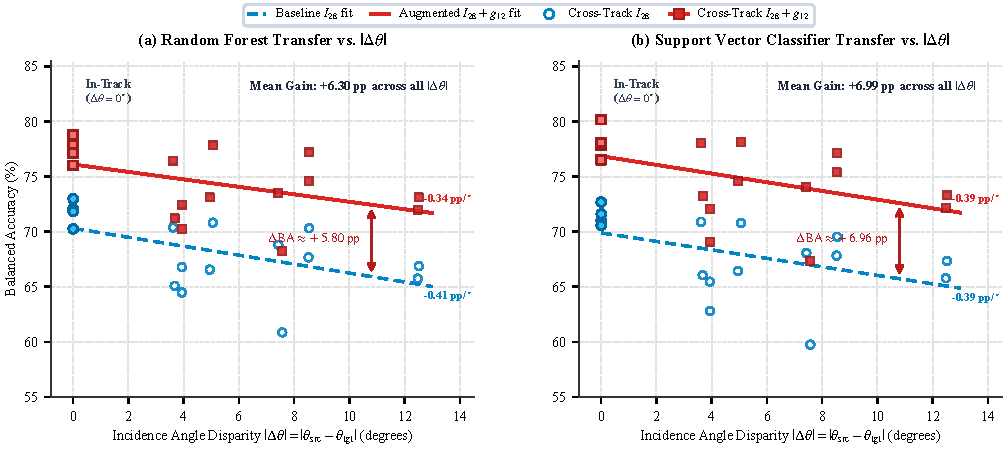
\includegraphics[width=0.98\textwidth]{fig12_angular_disparity.pdf}
\caption{Balanced accuracy against source--target incidence-angle separation for (a) RF and (b) SVC across sixteen track pairs. Baseline and augmented regression slopes are $-0.41$ and $-0.34\pp/^\circ$ for RF, and $-0.39$ and $-0.39\pp/^\circ$ for SVC. Lines summarize the observed track configurations.}
\label{fig:angular_disparity}
\end{figure}
\begin{figure}[H]
\centering
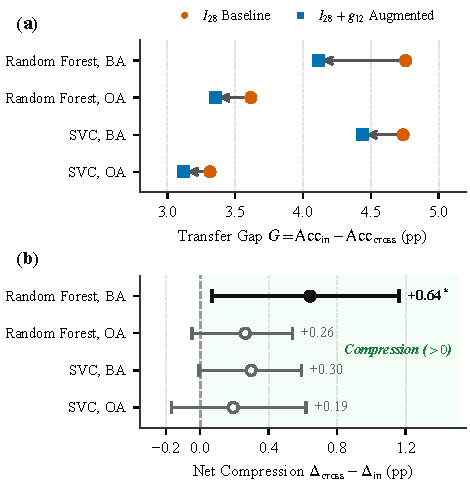
\includegraphics[width=0.48\textwidth]{fig13_transfer_gap_stabilization.pdf}
\caption{(a) In-track minus cross-track accuracy before and after coherence augmentation. (b) Paired gap reductions with 95\% joint block bootstrap intervals. The RF balanced-accuracy reduction is $+0.64\pp$ $[+0.07,+1.16]$; the other three intervals include zero.}
\label{fig:transfer_gap}
\end{figure}
\begin{figure}[H]
\centering
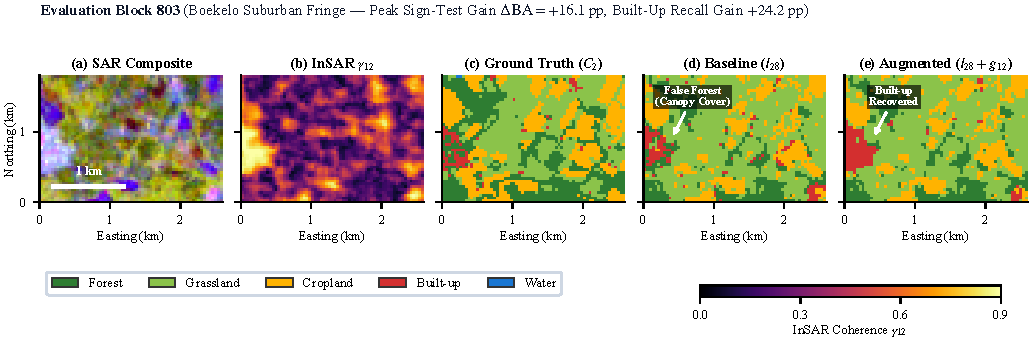
\includegraphics[width=0.98\textwidth]{fig9_multilandscape_error_resolution.pdf}
\caption{Spatial error resolution in suburban landscape under cross-track transfer ($\text{T}15 \to \text{T}37$, steep ascending to medium descending) in Block 803 (Boekelo suburban fringe, peak sign-test gain $\Delta\mathrm{BA} = +16.1\pp$): (a) SAR false-colour composite, (b) 12-day InSAR coherence $\gamma_{12}$, (c) harmonized consensus ground truth $C_2$, (d) baseline $I_{28}$ predictions misclassifying residential housing under canopy as forest (red outline), and (e) coherence-augmented $I_{28}{+}g_{12}$ predictions restoring the suburban core ($+24.2\pp$ local built-up recall gain; rural Block 603 exhibits an analogous $+37.5\pp$ gain).}
\label{fig:multilandscape_maps}
\end{figure}
\begin{figure}[H]
\centering
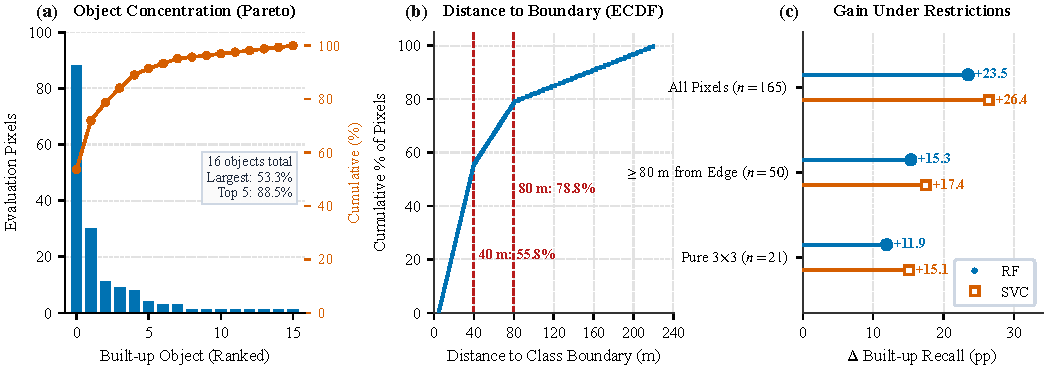
\includegraphics[width=0.98\textwidth]{fig10_label_audit.pdf}
\caption{Spatial support of the 165 built-up evaluation pixels. (a) Contributions of 16 connected objects; the largest supplies $53.3\%$ and the five largest $88.5\%$. (b) Distance to class boundaries. (c) Recall increments on interior and locally homogeneous subsets.}
\label{fig:labelaudit}
\end{figure}
\begin{figure}[H]
\centering
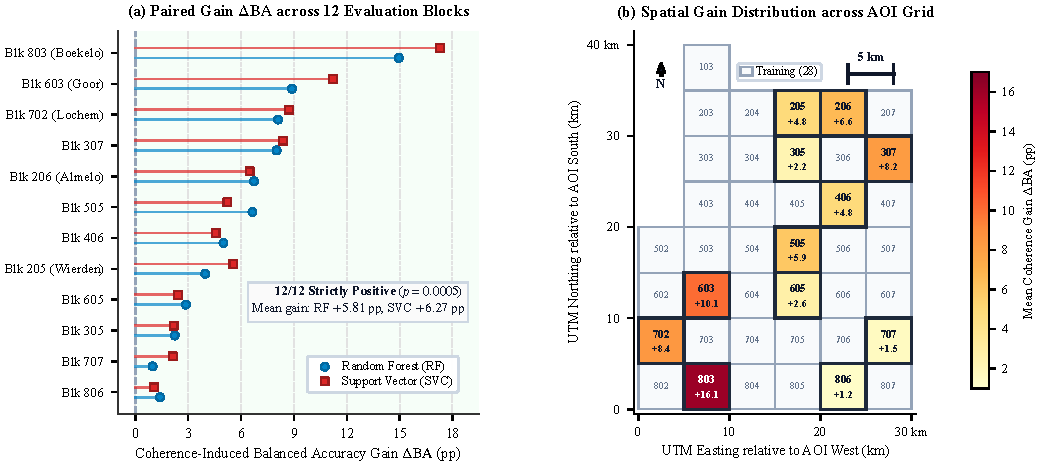
\includegraphics[width=0.98\textwidth]{fig11_spatial_sign_test.pdf}
\caption{Block-level coherence increments across twelve evaluation blocks. (a) RF and SVC increments, positive in all blocks for each learner (two-sided sign test, $p=0.0005$). (b) Spatial distribution of the mean increment, with training blocks shown for context.}
\label{fig:spatial_sign_test}
\end{figure}
\end{document}
